\documentclass[a4paper,11pt,oneside]{article}
%
% importar el archivo conf/packages.tex
\include{conf/packages}
%
% ===
% === Propiedades del documento: título, autor, etc
% ===
%
\newcommand{\titulo}{{\large FICH --- UNL}\\
  Auditoría Informática -- 2010\\
  {Trabajo Final, Etapa 1: Presentación de la Organización}}
\newcommand{\autor}{Galarza, Romina \and Mastaglia, Nicolás \and Torrez, Mauro}
\newcommand{\fecha}{\today}
\newcommand{\tituloPDF}{Auditoría}
\newcommand{\autorPDF}{Mauro Torrez}
\newcommand{\asuntoPDF}{MNS GTP2}
\newcommand{\clavesPDF}{MNS GTP2}
%
% importar los archivos conf/config.tex y conf/comandos.tex
\include{conf/config}
\include{conf/comandos}
%% Serif .......................................................................
%%
%% New Century Schoolbook
%% \usepackage[T1]{fontenc}
%% \usepackage{fouriernc}
%%
%%
%% TeX Gyre Schola (New Century extendida)
%% \usepackage[T1]{fontenc}
%% \usepackage{tgschola}
%%
%%
%% Utopia
%% \usepackage[T1]{fontenc}
%% \usepackage{fourier}
%%
%%
%% Utopia (con MathDesign)
%% \usepackage[T1]{fontenc}
%% \usepackage[adobe-utopia]{mathdesign}
%%
%%
%% Computer Concrete
%% \usepackage[T1]{fontenc}
%% \usepackage{concmath}
%%
%%
%% Charter BT
%% \usepackage[T1]{fontenc}
%% \usepackage[bitstream-charter]{mathdesign}
%%
%%
%% Nimbus Roman (clon de Times)
%% \usepackage[T1]{fontenc}
%% \usepackage{nimbus}
%%
%%
%% TeX Gyre Termes (version mejorada de Nimbus Roman)
%% \usepackage[T1]{fontenc}
%% \usepackage{tgtermes}
%%
%%
%% GFS Bodoni
%% \usepackage[T1]{fontenc}
%% \usepackage[default]{gfsbodoni}
%%
%%
%% Baskervald ADF
%% \usepackage[T1]{fontenc}
%% \usepackage{baskervald}
%%
%%
%% Efont Serif -- descargar de http://openlab.jp/efont/serif/
%% \usepackage[T1]{fontenc}
%% \usepackage{efont,mathesf}
%% \renewcommand*\oldstylenums[1]{{\fontfamily{esfod}\selectfont#1}}
%%
%%
%%
%%
%%
%% Sans-Serif ..................................................................
%%
%%
%% Optima (clon de, URW Classico)
%% \usepackage[T1]{fontenc}
%% \renewcommand*\sfdefault{uop}
%%
%%
%% Avantgarde (clon de, URW Gothic)
%% \usepackage[T1]{fontenc}
%% \usepackage{avant}
%%
%%
%% TeX Gyre Adventor (version mejorada de Avantgarde)
%% \usepackage[T1]{fontenc}
%% \usepackage{tgadventor}
%%
%%
%% Nimbus Sans (clon de Helvetica)
%% \usepackage[T1]{fontenc}
%% \usepackage{nimbus}
%%
%%
%% Helvetica (clon de, Nimbus Sans)
%% \usepackage[T1]{fontenc}
%% \usepackage[scaled]{helvet}
%%
%%
%% TeX Gyre Heros (version mejorada de Nimbus Sans)
%% \usepackage[T1]{fontenc}
%% \usepackage{tgheros}
%%
%%
%% Boilinum
\usepackage[T1]{fontenc}
\usepackage{libertine}
%%
%%
%% Computer Modern Bright
%% \usepackage[T1]{fontenc}
%% \usepackage{cmbright}
%%
%%
%% Latin Modern Sans
%% \usepackage[T1]{fontenc}
%% \usepackage{lmodern}
%%
%%
%% Epigrafica
%% \usepackage[OT1]{fontenc}
%% \usepackage{epigrafica}
%%
%%
%%
%% Si quiero el documento en sans en vez de Roman:
%% \renewcommand*\familydefault{\sfdefault}
%% ...............................................
%% 
%%
%%
%% Monospaced ..................................................................
%%
%%
%% Pandora Typewriter
%% \usepackage[T1]{fontenc}
%% \usepackage{pandora}
%%
%%
%% Letter Gothic
%% \usepackage[T1]{fontenc}
%% \usepackage{ulgothic}
%%
%%
%% Inconsolata
%% \usepackage[T1]{fontenc}
%% \usepackage{inconsolata}
%%

%
% ===
% === Inicio del documento
% === 
%
\begin{document}
% crear la página de título
\maketitle
%
%\tit*{Etapa}
%
\section{Presentación de la organización}
%
Realizaremos el trabajo de auditoría en Rectorado de la Universidad
Nacional del Litoral.

El Rectorado, es el lugar físico en donde se encuentran situados las
estructuras administrativas y gubernamentales de la Universidad
Nacional del Litoral. 
Su actividad es básicamente administrativa y de gestión, y su estructura
se compone de una serie de secretarías enfocadas a algún área en
paticular.

En la figura \ref{organi-rectorado} vemos un esquema básico de esta
estructura.
%
\begin{figure}
  \center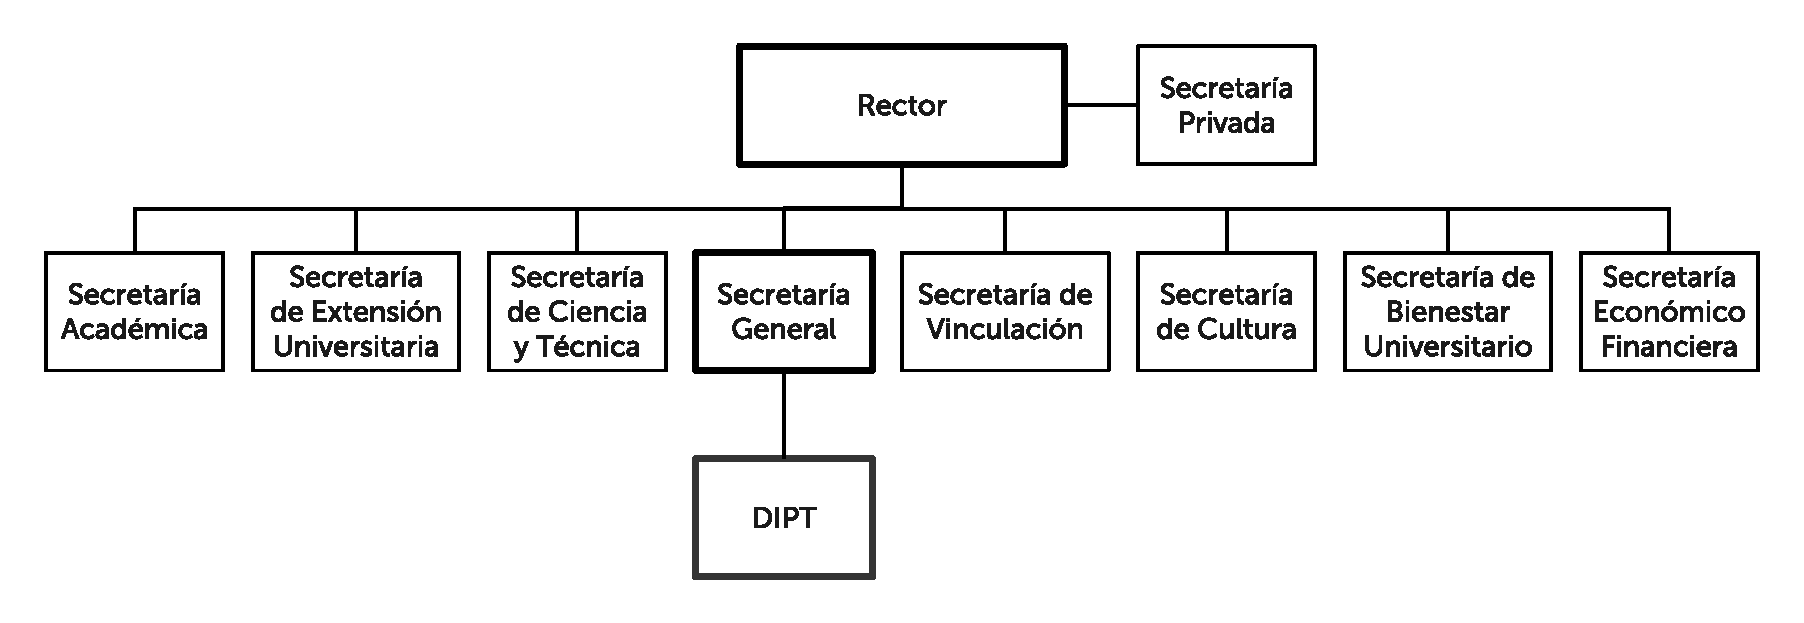
\includegraphics[width=127mm]{img/organi_rectorado}
  \caption{Organigrama del Rectorado}
  \label{organi-rectorado}
\end{figure}
%
\section{El área de sistemas de información}
%
El area de sistemas de información es la Dirección de Informatización
y Planificación Tenológica la cual se encarga de llevar a cabo las
tareas de desarrollo, mantenimiento y administracion de recursos
informáticos, servidores, aplicaciones y soporte técnicos a los
usuarios finales en el rectorado.

Jerárquicamente, esta dirección depende de la Secretaría General.
%
\subsection{Estructura}
%
La DIPT cuenta con unos 30 empleados, y se subdivide en los siguientes
áreas, como se muestra en la figura \ref{organi-dipt}:
\begin{description}
\item[Cómputos]
  Se encarga del desarrollo, mantenimiento y soporte técnico del
  sistema de gestión de personal SIU Pampa y de la impresión de los
  recibos de sueldo.
%
\item[Desarrollo]
  Su función se basa en el desarrollo, mantenimiento y soporte técnico
  de los sistemas contable SIU Pilagá, de gestión de alumnos SIU
  Guaraní, entre otros.
%
\item[Administración]
  Se ocupa de la implementación y del correcto funcionamiento de los
  servidores (correo, web, sistemas, etc) y la compra de equipamiento
  de red y servidores.
%
\item[Seguridad]
  Se encarga de la inspección y revisión de la seguridad de los
  sistemas y redes.
%
\item[Soporte técnico]
  Este sector provee asistencia técnica a los usuarios en sus puestos
  de trabajo.
\end{description}
%
\begin{figure}
  \center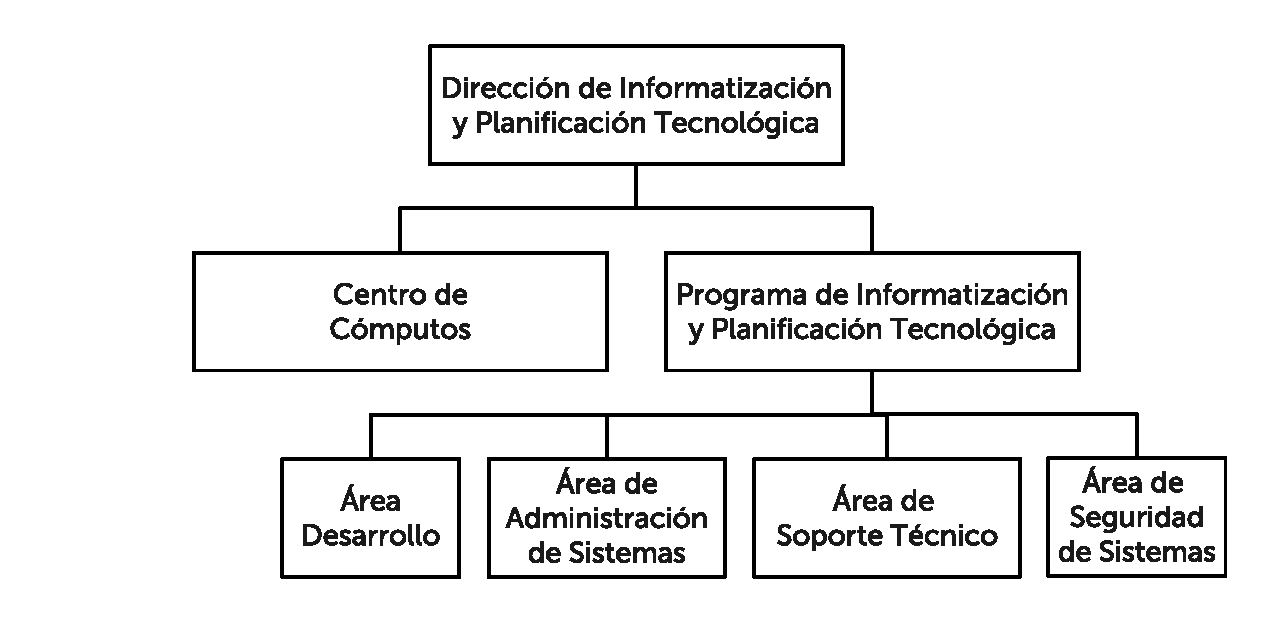
\includegraphics[width=127mm]{img/organi_dipt}
  \caption{Organigrama de la DIPT}
  \label{organi-dipt}
\end{figure}
%
\section{Estrategias informáticas a corto, mediano y largo plazo}
%
La planificacion de las estrategias infomáticas se da mayormente en la
parte de administración junto con el director de la Dirección.

Entre las estrategias a corto plazo podemos citar:
%
\begin{description}
\item[Mantenimiento y soporte al usuario:]
  Día a día se proograman actividades de mantenimiento en los sistemas
  llevadas a cabo principalmente por el área de administración, y de
  mantenimiento y resolución de problemas en las estaciones de trabajo
  efectuadas por Soporte técnico.
\end{description}
Entre las estrategias a mediano plazo podemos citar:

\begin{description}
\item[Plan de contingencia ante fallas eléctricas:]
  Se está desarrollando actualmente y consiste en la instalación de un
  UPS y un grupo electrógeno para evitar la caíde de los servidores en
  caso de un eventual corte de energía.
%
\item[Migración y actualización del servidor de correo]
  Consiste en la instalación de un nuevo servidor, y el traspaso de
  datos desde el servidor actual.
%
\item[Proyecto ``/oficina'':]
  Este proyecto pretende en brindar a las distintas oficinas del
  rectorado, su propio espacio web tanto en la intranet como en
  internet, a través de un CMS (\eng{Content Management System})
  brindándole mejoras en la administración, compartición y publicación
  de documentos.
\end{description}
%
No existen planificación definida a realizar en el largo plazo.
%
\section{Hardware}
%
El hardware que esta disponible en rectorado esta inventariado por la
Dirección de Patrimonio, externa a la DIPT.

A continuación, se presenta un resumen del hardware con que cuenta el
rectorado en su edificio principal.
%
\subsection*{Piso 3}
%
En este piso encontramos la DIPT y la oficina de Personal.
%
\subsubsection*{DIPT}
%
\begin{itemize*}
\item 27 workstations
\item 2 notebooks
\item 2 impresoras
\item 1 multifución
\item 5 teléfonos
\item 5 aires acondicionados
\item 1 cañón
\end{itemize*}
%
A su vez dentro de la DIPT encontramos la sala de servidores que cuenta con:
\begin{itemize*}
\item 1 router raíz
\item 2 switches raiz
\item 1 aire acondicionado
\item 2 racks con servidores
\item 1 UPS por rack
\end{itemize*}
%
\subsubsection*{Personal}
\begin{itemize*}
\item 20 workstations
\item 6 impresoras
\item 1 multifución
\item 9 teléfonos
\item 2 aires acondicionados
\end{itemize*}
%
\subsection*{Piso 2}
%
\subsubsection*{DGA}
\begin{itemize*}
\item 26 workstations
\item 16 impresoras
\item 1 multifución
\item 16 teléfonos
\item 3 aires acondicionados
\item 3 switches
\item 2 fax
\end{itemize*}
%
\subsubsection*{Despacho General, Consejo Superior}
\begin{itemize*}
\item 10 workstations
\item 4 impresoras
\item 4 teléfonos
\item 1 aire acondicionado
\item 1 switch
\item 1 fax
\end{itemize*}
%
\subsection*{Piso 1}
%
\subsubsection*{Ala este}
\begin{itemize*}
\item 26 workstations
\item 16 impresoras
\item 1 multifución
\item 16 teléfonos
\item 3 aires acondicionados
\item 3 switches
\item 2 fax
\end{itemize*}
%
\subsubsection*{Ala oeste}
\begin{itemize*}
\item 10 workstations
\item 4 impresoras
\item 4 teléfonos
\item 1 aire acondicionado
\item 1 switch
\item 1 fax
\end{itemize*}
%
\subsection*{Planta baja}
%
\subsubsection*{Ala este}
\begin{itemize*}
\item 26 workstations
\item 16 impresoras
\item 1 multifución
\item 16 teléfonos
\item 3 aires acondicionados
\item 3 switches
\item 2 fax
\end{itemize*}
%
\subsubsection*{Ala oeste}
\begin{itemize*}
\item 10 workstations
\item 4 impresoras
\item 4 teléfonos
\item 1 aire acondicionado
\item 1 switch
\item 1 fax
\end{itemize*}
%
\section{Software}
%
\subsection{Software base}
%
\subsubsection*{Sistema operativo}
Tanto en el Rectorado como en la DIPT, se utiliza principalmente el
sistema operativo Debian GNU/Linux y en menor medida Microsoft Windows
XP. En las notebooks personales de los usuarios tambien podemos
encontrar Microsoft Windows Vista y Windows 7.
%
\subsubsection*{Antivirus}
En esta organización no posee un antivirus preestablecido, el más
utilizado es el Avira Free Editionque es el que instala el personal de
soporte técnico en las máquinas de los usuarios, también encontramos
el AVG y el Nod 32, entre otros.
%
\subsubsection*{Base de datos}
%
Tanto en los sistemas desarrollados internamente como en los del SIU
se utiliza PostgresSQL como motor de base de datos principal.
%
\subsection*{Software aplicativo}
%
\subsubsection*{Software de programación}
%
Para el desarrollo de los sistemas propios se utiliza principalmente el lenguaje Java, y el software de SIU esta desarrollado principalmente en PHP. Tambien encontramos sistemas en ASP.

Las IDEs que se utilizan son Netbeans, Eclipse y GNU Emacs.

Se utiliza el sistema de versionado de código SVN mantenido por los administradores en un respositorio centralizado en los servidores propios.

\section{Esquema de telecomunicaciones}

\section{Normativa Interna}
%
Existen determinadas normativas respecto del uso de la red, impuestas
desde arriba desde el CETUL, que es el órgano encargado del manejo e
interconexión desde la Universidad a Internet y otras redes externas,
y provee de conexión a las diferentes instituciones de la UNL.

Los usuarios deben firmar un acuerdo de conformidad tanto al solicitar
la creación de una cuenta de correo de rectorado, como al requerir la
habilitación de una nueva computadora en la red.

Algunos de los puntos de este acuerdo de conformidad establecen lo
siguiente:
%
\begin{itemize*}
\item Prohibición de utilizar los servicios de la red para uso
  comercial particular,
\item Prohibición del uso de la red con fnes de hackeo/cracking, y
  difusión de virus/spyware/malware
\item Prohibición de la utilización de la cuenta de correo electrónico
  para envío de spam
\end{itemize*}
%
\subsection*{Procedimientos internos de la DIPT}
%
\begin{description}
\item[Atención a usuarios:] el siguiente esquema se sigue para brindar
  soporte técnico a los usuarios:
  \begin{enumerate*}
  \item Los usuarios inician una solicitud de soporte técnico llamando
    a un número telefónico dispuesto a tal efecto.
  \item Se asigna un número de caso completando un "ticket" en un
    sistema de seguimiento.
  \item El técnico se encarga de revisar la lista de tareas
    pendientes, asignándose de la lista para atender el caso,
    realizando un seguimiento en el sistema por cada uno.
  \item Una vez resuelto el problema, se cierra el caso en el sistema.
  \end{enumerate*}
\item[Tickets:] el sistema de tickets es utilizado por casi todos los
  sectores del área, siendo a través de este sistema la forma más
  común entre los distintos sectores del área de Informática.
\item[Software libre:] salvo casos excepcionales, la política de
  rectorado establece que sólo se utilizará software libre en las
  estaciones de trabajo.
\item[Software del SIU:] la UNL adhiere al consorcio SIU, lo que
  implica que la mayoría de los sistemas de la Universidad provienen
  de SIU.
\end{description}
%
\section{Relaciones con terceros}

\section{Politicas de selección, capacitación y entrenamiento de personal}

No existen políticas específicas para la selección del personal más allá de la idoneidad, experiencia, etc.

\section{Identificacion de problemas, necesidades e incertidumbres existentes en la organización}
\end{document}
